\chapter{Diseño e implementación} % Main chapter title

\label{Chapter3}

Este capítulo describe en detalle el sistema implementado, sus partes y su interacción, incluyendo los criterios adoptados durante el proceso de desarrollo. Luego se explica qué sensores se utilizaron y su funcionamiento, qué componentes fueron utilizados para el circuito impreso. Y, finalmente, describe el funcionamiento y el proceso de desarrollo del software utilizado en la parte adquisidora y la interfaz gráfica.

\section{Descripción del sistema implementado}

La parte adquisidora del sistema se implementó sobre una placa de desarrollo EDU-CIAA debido a la experiencia de uso acumulada durante el cursado de la Especialización en Sistemas Embebidos. Además, el microprocesador que utiliza esa placa de desarrollo, el NXP LPC4337, cuenta con los periféricos necesarios para digitalizar las señales de todos los sensores a utilizar y enviar los datos recolectados al módulo de comunicación \textit{Bluetooth}. Específicamente el microprocesador posee: interfaz SPI de cuatro canales con velocidad hasta 60MB por segundo; interfaz USART y tres conversores analógico digital de 10 bits de resolución, y tasa de muestreo de 400 mil muestras por segundo. El circuito de alimentación, digitalización de las señales de los sensores y comunicación con el módulo \textit{Bluetooth} se diseñó para funcionar como "Poncho"  \cite{poncho} de la EDU-CIAA.

Para la comunicación \textit{Bluetooth} entre las partes se utilizó el módulo HM-10, basado en el circuito integrado CC2541 de Texas Instruments. Se utilizó este módulo porque sus niveles de señales son compatibles con los de la EDU-CIAA, tiene un bajo consumo de energía y puede transmitir información serie con una velocidad de hasta 6 kilobytes por segundo \cite{HM-10}.

Para la interfaz gráfica se utilizó una \textit{Raspberry Pi 3B+} con una pantalla LCD táctil capacitiva de 5 pulgadas de longitud diagonal y resolución de 800 píxeles de ancho por 480 píxeles de alto. Se eligió esta plataforma porque posee comunicación \textit{Bluetooth Low-Energy}, utiliza un sistema operativo basado en Linux y puede correr scripts escritos en Python 3.7 \cite{raspberrypi}. Como el software de la interfaz gráfica fue desarrollado enteramente en Python 3.7, el dispositivo para la interfaz gráfica podría ser cualquiera que cumpla con las especificaciones nombradas.

\section{Desarrollo del circuito impreso} \label{circuito}

Para el prototipo se desarrolló un circuito impreso que funciona como "poncho" para la EDU-CIAA. Un poncho es un circuito impreso con conectores específicos para conectarse a la EDU-CIAA y acceder a sus señales. El diseño del circuito se hizo con el software KiCAD versión 6.

\subsection{Circuito de medición de temperatura}

Para medir las temperaturas de los gases de admisión, escape y temperatura de aceite se utilizaron termocuplas tipo K. Una termocupla es un dispositivo compuesto por dos alambres metálicos de distintos materiales unidos en un extremo. Cuando existe una diferencia de temperatura entre sus extremos se genera una diferencia de tensión en el extremo abierto, la tensión generada es proporcional a la diferencia de temperatura, a este efecto se llama efecto Seebeck \cite{termocupla}.

Para convertir la tensión de la termocupla en un valor de temperatura se utilizó el circuito integrado MAX31855K. Este integrado digitaliza la señal de termocuplas tipo K en un rango entre -200 \degree C y 700 \degree C con una resolución de 0,25 \degree C. Su interfaz es SPI de solo lectura y tiene una velocidad máxima de muestreo de 1 kHz. Además de informar la lectura de temperatura también comunica códigos de error si la termocupla esta desconectada, o en cortocircuito con la alimentación o masa \cite{MAX31855}. Con estas características se cumplen los requisitos REQ-ADQ-001 y REQ-ADQ-002. En total se utilizaron en el circuito impreso tres de estos circuitos integrados, uno para cada termocupla.

\subsection{Sensor de velocidad de giro}

Para medir la velocidad de giro del cigüeñal del motor se utilizó un sensor de reluctancia variable. Estos sensores convierten variaciones en la reluctancia magnética en una señal de tensión. Estos variaciones son generadas por la presencia o movimiento de un objeto ferroso en la proximidad del sensor. La medición de la velocidad de giro del cigüeñal se hace a través de una rueda fónica. Una rueda fónica es una rueda dentada de acero que gira en conjunto con el cigüeñal del motor. Cuando la rueda gira los dientes se acerca al sensor y se alejan al sensor y esto genera un tren de pulsos en sus bornes. Para medir la velocidad de giro la señal del sensor tiene que ser convertida a una señal cuadrada de valores dentro del rango admisible por el microprocesador. Para esto se utilizó el circuito integrado MAX9924 \cite{MAX9924}. El proceso de adaptación de la señal del MAX9924 está representado en el diagrama de bloques de la figura \ref{fig:bloq-9924}.

\break

\begin{figure}[htpb]
\centering
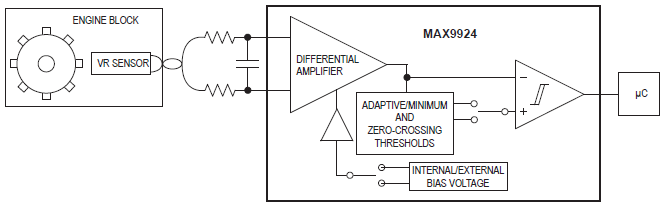
\includegraphics[width=.9\textwidth]{./Figures/max9924.png}
\caption{Funcionamiento del MAX9924 representado en diagrama de bloques. \protect\footnotemark[3].}
\label{fig:motor-combustion}
\end{figure}
\footnotetext[3]{Imagen tomada de \cite{MAX9924}}


\subsection{Circuito de medición de variables analógicos}

Las variables analógicas son las variables generadas por los sensores lambda, presión de aceite y la tensión de la batería. Para digitalizar estas señales se utilizaron el conversor analógico digital de la ECU-CIAA con sus tres canales independientes.

\section{Desarrollo del firmware}

Descripción de criterios y consideraciones elegidas para el desarrollo del firmware.

\section{Desarrollo de la interfaz gráfica}

Descripción de criterios y consideraciones elegidas para el desarrollo de la interfaz gráfica.

